\chapter{Implementación}
Después de decidir las características de las que dispondrá \jj es necesario analizar como se implementaran estas. Por el lado de \cc tenemos que las interfaces que definen el comportamiento de las clases que contendrán a las sentencias SQL comparten muchas cosas por lo que hay que analizar adecuadamente las herencias y definición de interfaces. Elegir adecuadamente la estructura del proyecto puede hacer la diferencia entre una librería\footnote{como lo defino al final!!!!!!} mantenible y ampliable contra una pila de código difícil de entender. Así que como en el capitulo anterior analizaremos \jj por secciones  primero la sección que se encarga de manejar la conexión con la base de datos y después la que se encarga de abstraer el uso de SQL.






\section{Implementación de el envoltorio de \jj}

A few words




\section{Implementación de \cc}

Para la implementación de las especificaciones declaradas anteriormente nos encontramos con que existen algunas similitudes entre las diferentes clases definidas anteriormente, atendiendo a que cada clase representa a una de las sentencias SQL que se incluyeron en el proyecto y cada clase esta compuesta por:
\begin{itemize}
\item Variables que almacenaran los datos necesarios para la construcción de los métodos.

\item Métodos para inicializar la clase y agregar (lo que comúnmente se dice\textit{setear}), es decir poblarla con los datos necesarios para su construcción.

\item Métodos para armar la sentencia.

\end{itemize}

La \Figpage{fig:query} muestra la forma en la que se constituye 

\begin{figure}
  \centering
    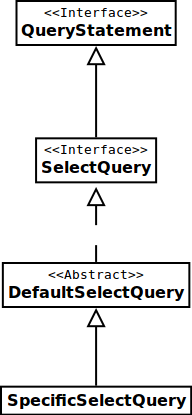
\includegraphics[width=0.2\textwidth]{figuras/crossdb-query.png}
  \caption{Mi Figura}
  \label{fig:query}
\end{figure}
algo aca
\begin{figure}
  \centering
    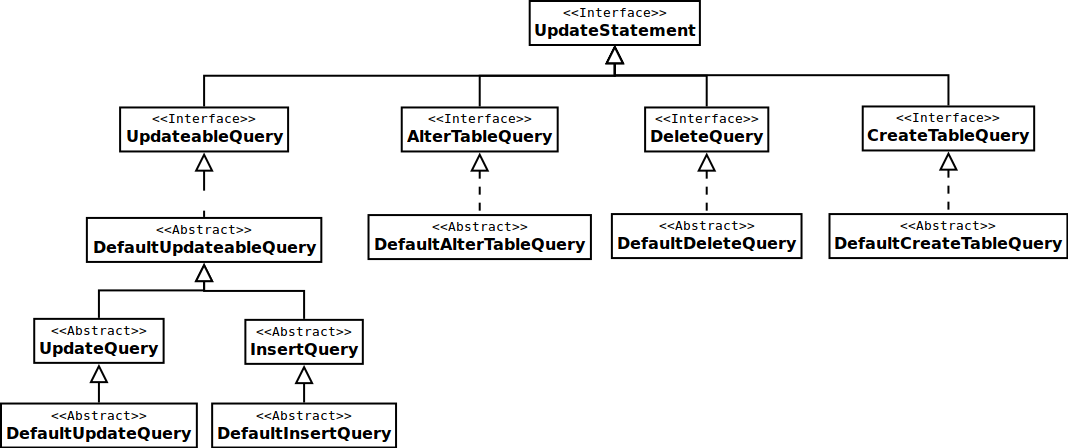
\includegraphics[width=\textwidth]{figuras/crossdb-update.png}
  \caption{Mi Figura}
  \label{fig:update}
\end{figure}

Que se convertirá en una interfaz como la siguiente:


\begin{lstlisting}[title=Pseudocódigo interfaz para CREATE]
class CreateStatement{
	setTable(name);
	setTable(name, databaseName);
	addColumn(columnName, value);
	addWhereClause(whereClause);
}
\end{lstlisting}
